\chapter*{EDHEC 2017 : le sujet}
  
%

\section*{Exercice 1}

\noindent
On considère la fonction $f$ qui à tout couple $(x,y)$ de $\R^{2}$
associe le réel :
\[
f(x,y) = x^{4} + y^{4} - 2 \ (x-y)^{2}
\]
\begin{noliste}{1.}
  \setlength{\itemsep}{4mm}
\item Justifier que $f$ est de classe $\Cont{1}$ sur $\R^{2}$.

  

\item
  \begin{noliste}{a)}
    \setlength{\itemsep}{2mm}
  \item Calculer les dérivées partielles d'ordre $1$ de $f$.

    

  \item Montrer que le gradient de $f$ est nul si, et seulement si, on
    a : $ \left\{
      \begin{array}{rcl}
        x^{3}-x + y & = & 0 \\
        y^{3} + x-y & = & 0
      \end{array}
    \right.$.

    

  \item En déduire que $f$ possède trois points critiques : $(0,0)$,
    $(\sqrt{2},-\sqrt{2}), (-\sqrt{2},\sqrt{2})$.

    
  \end{noliste}


%\newpage


\item
  \begin{noliste}{a)}
    \setlength{\itemsep}{2mm}
  \item Calculer les dérivées partielles d'ordre 2 de $f$.

    

  \item Écrire la matrice hessienne de $f$ en chaque point critique.

    
    

    %\newpage


  \item Déterminer les valeurs propres de chacune de ces trois
    matrices puis montrer que $f$ admet un minimum local en deux de
    ses points critiques. Donner la valeur de ce minimum.

    

  \item Déterminer les signes de $f(x,x)$ et $f(x,-x)$ au voisinage de
    $x = 0$. \\
    Conclure quant à l'existence d'un extremum en le troisième point
    critique de $f$.

    
  \end{noliste}
  
\item
  \begin{noliste}{a)}
    \setlength{\itemsep}{2mm}
  \item Pour tout $(x,y)$ de $\R^{2}$, calculer $f(x,y) -
    (x^{2}-2)^{2} - (y^{2}-2)^{2} - 2(x + y)^{2}$.

    


    %\newpage


  \item Que peut-on déduire de ce calcul quant au minimum de $f$ ?

    

  \end{noliste}

\item
  \begin{noliste}{a)}
    \setlength{\itemsep}{2mm}
  \item Compléter la deuxième ligne du script suivant afin de définir
    la fonction $f$.
    \begin{scilab}
      & \tcFun{function} \tcVar{z} = \underline{f}(\tcVar{x},\tcVar{y})
      \nl %
      & \qquad \tcVar{z} = ------ \nl %
      & \tcFun{endfunction} \nl %
      & x = linspace(-2,2,101) \nl %
      & y = x \nl %
      & fplotd3d(x,y,f)
    \end{scilab}
    
    
    
  \item Le script précédent, une fois complété, renvoie l'une des
    trois nappes suivantes. Laquelle ? \\
    Justifier la réponse.
    \[
    \begin{array}{C{4.5cm}@{\qquad}C{4.5cm}@{\qquad}C{4.5cm}}
      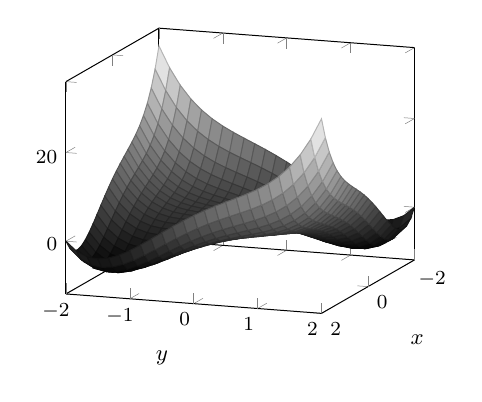
\begin{tikzpicture}[scale=.9]
        \begin{axis}[
          colormap/blackwhite,
          % title={$x \exp(-x^2-y^2)$},
          % rotate = 180,
          xlabel=$x$, ylabel=$y$, %
          % xlabel style = {rotate = -90}, %
          small, %
          view = {110}{15}, %
          ] %
          \addplot3[ %
          surf, %
          domain=-2:2, %
          domain y=-2:2, %
          ] %
          {x^4 + y^4 - 2*(x-y)^2}; %
        \end{axis}
      \end{tikzpicture}
      & 
      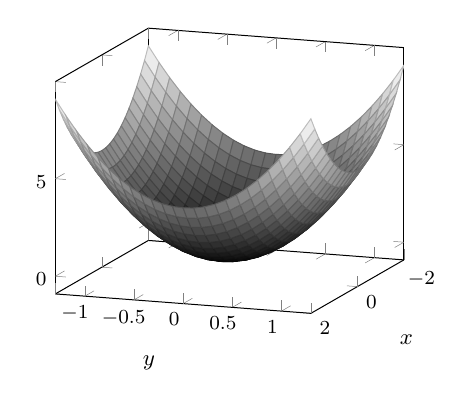
\begin{tikzpicture}[scale=.9]
        \begin{axis}[
          colormap/blackwhite,
          % title={$x \exp(-x^2-y^2)$},
          xlabel=$x$, ylabel=$y$, %
          small, %
          view = {110}{15}, %
          ] %
          \addplot3[ %
          surf, %
          domain=-2:2, %
          domain y=-1.3:1.3, %
          ] %
          {x^2 + 3 * y^2}; %
        \end{axis}
      \end{tikzpicture}
      &
      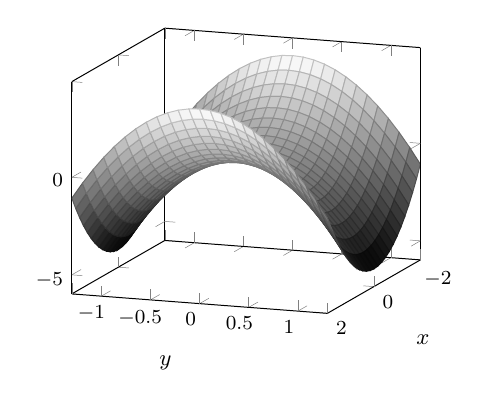
\begin{tikzpicture}[scale=.9]
        \begin{axis}[
          colormap/blackwhite,
          % title={$x \exp(-x^2-y^2)$},
          xlabel=$x$, ylabel=$y$, %
          small, %
          view = {110}{15}, %
          ] %
          \addplot3[ %
          surf, %
          domain=-2:2, %
          domain y=-1.3:1.3, %
          ] %
          {x^2-3*y^2}; %
        \end{axis}
      \end{tikzpicture}
      \nl
      Nappe $1$ & Nappe $2$ & Nappe $3$
    \end{array}
    \]
    
    
    %\newpage
    
    
    
  \end{noliste}
\end{noliste}


\newpage


\section*{Exercice 2}

\noindent
On note $E$ l'espace vectoriel des fonctions polynomiales de degré
inférieur ou égal à $2$ et on rappelle que la famille
$(e_{0},e_{1},e_{2})$ est une base de $E$, les fonctions $e_{0}$,
$e_{1}$ $e_{2}$ étant définies par :
\[
\forall t \in \R \quad e_{0}(t) = 1, \quad e_{1}(t) = t, \quad
e_{2}(t) = t^{2}
\]
On considère l'application $\varphi$ qui, à toute fonction $P$ de $E$,
associe la fonction, notée $\varphi(P)$, définie par :
\[
\forall x \in \R, \ \left(\varphi(P)\right)(x) = \dint{0}{1} P(x + t)
\ dt
\]
\begin{noliste}{1.}
 \setlength{\itemsep}{4mm}
\item
  \begin{noliste}{a)}
    \setlength{\itemsep}{2mm}
  \item Montrer que $\varphi$ est linéaire.

    
    
  \item Déterminer $\left(\varphi(e_{0})\right)(x)$,
    $\left(\varphi(e_{1})\right)(x)$ et
    $\left(\varphi(e_{2})\right)(x)$ en fonction de $x$, puis écrire
    $\varphi(e_{0})$, $\varphi(e_{1})$ et $\varphi(e_{2})$ comme
    combinaison linéaire de $e_{0}$, $e_{1}$ et $e_{2}$.

    

  \item Déduire des questions précédentes que $\varphi$ est un
    endomorphisme de $E$.

    
  \end{noliste}
  
  
  %\newpage
  
  
\item
  \begin{noliste}{a)}
    \setlength{\itemsep}{2mm}
  \item Écrire la matrice $A$ de $\varphi$ dans la base
    $(e_{0},e_{1},e_{2})$. On vérifiera que la première ligne de $A$
    est :
    \[
    \begin{smatrix}
      1 & \dfrac{1}{2} & \dfrac{1}{3}
    \end{smatrix}
    \]

    

  \item Justifier que $\varphi$ est un automorphisme de $E$.

    

  \item L'endomorphisme $\varphi$ est-il diagonalisable ?

    
  \end{noliste}

\item Compléter les commandes \Scilab{} suivantes pour que soit
  affichée la matrice $A^{n}$ pour une valeur de $n$ entrée par
  l'utilisateur :
  \begin{scilab}
    & n = input(\ttq{}entrez une valeur pour n : \ttq{}) \nl %
    & A = [------] \nl %
    & disp(------)
  \end{scilab}

  


%\newpage


\item
  \begin{noliste}{a)}
    \setlength{\itemsep}{2mm}
  \item Montrer par récurrence que, pour tout entier naturel $n$, il
    existe un réel $u_{n}$ tel que l'on ait :
    \[
    A^{n} = 
    \begin{smatrix}
      1 & \frac{n}{2} & u_{n}\\
      0 & 1 & n\\
      0 & 0 & 1
    \end{smatrix}
    \]
    Donner $u_{0}$ et établir que : $\forall n \in \N, \ u_{n + 1} =
    u_{n} + \dfrac{1}{6}\left(3n + 2\right)$.
    
    

  \item En déduire, par sommation, l'expression de $u_{n}$ pour tout
    entier $n$.

    

  \item Écrire $A^{n}$ sous forme de tableau matriciel.

    
  \end{noliste}
\end{noliste}


%\newpage


% \section*{Exercice 3}

% \noindent
% Soit $V$ une variable aléatoire suivant la loi exponentielle de
% paramètre $1$, dont la fonction de répartition est la fonction $F_{V}$
% définie par : $F_{V}(x) = \left\{
% \begin{array}{cl}
% 0 & \hbox{ si } x \leq 0\\
% 1-\ee^{-x} & \hbox{ si } x>0
% \end{array}
% \right.$.\\
% On pose $W = -\ln(V)$ et on admet que $W$ est aussi une variable
% aléatoire dont le fonction de répartition est notée $F_{W}$. On dit
% que $W$ suit une loi de Gumbel.
% \begin{noliste}{1.}
%   \setlength{\itemsep}{4mm}
% \item
%   \begin{noliste}{a)}
%     \setlength{\itemsep}{2mm}
%   \item Montrer que : $\forall x \in \R, \ F_{W}(x) =
%     \ee^{-\ee^{-x}}$.
%   \item En déduire que $W$ est une variable à densité.
%   \end{noliste}
% \end{noliste}

% \begin{noliste}{$\sbullet$}
% \item On désigne par $n$ un entier naturel non nul et par $X_{1},
%   \ldots, X_{n}$ des variables aléatoires définies sur le même espace
%   probabilisé, indépendantes et suivant la même loi que $V$, c'est à
%   dire la loi $\Exp{1}$.

% \item On considère la variable aléatoire $Y_{n}$ définie par $Y_{n} =
%   \max(X_{1},X_{2}, \ldots,X_{n})$, c'est à dire que pour tout
%   $\omega$ de $\Omega$, on a : $Y_{n}(\omega) =
%   \max(X_{1}(\omega),X_{2}(\omega), \ldots, X_n(\omega))$.\\
%   On admet que $Y_{n}$ est une variable aléatoire à densité.
% \end{noliste}

% \begin{noliste}{1.}
%   \setlength{\itemsep}{4mm} %
%   \setcounter{enumi}{1}
% \item
%   \begin{noliste}{a)}
%     \setlength{\itemsep}{2mm}
%   \item Montrer que la fonction de répartition $F_{Y_{n}}$ de $Y_{n}$
%     est définie par :
%     \[
%     F_{Y_{n}}(x) \left\{
%       \begin{array}{cl}
%         0 & \hbox{ si } x<0\\
%         (1-\ee^{-x})^{n} & \hbox{ si } x \geq 0
%       \end{array}
%     \right.
%     \]
%   \item En déduire une densité $f_{Y_{n}}$ de $Y_{n}$.
%   \end{noliste}
  
% \item
%   \begin{noliste}{a)}
%     \setlength{\itemsep}{2mm}
%   \item Donner un équivalent de $1-F_{Y_{n}}(t)$ lorsque $t$ est au
%     voisinage de $ + \infty$, puis montrer que l'intégrale $
%     \dint{0}{+ \infty} \left(1-F_{Y_{n}}(t) \right) \ dt$ est
%     convergente.
%   \item Établir l'égalité suivante :
%     \[
%     \forall x \in \R^+, \ \dint{0}{x} (1-F_{Y_{n}}(t)) \ dt =
%     x\left(1-F_{Y_{n}}(x)\right) + \dint{0}{x} t f_{Y_{n}}(t) \ dt
%     \]
%   \item Montrer que :$ \dlim{ x \to + \infty}
%     x\left(1-F_{Y_{n}}(x)\right) = 0$.
%   \item En déduire que $Y_{n}$ possède une espérance et prouver
%     l'égalité :
%     \[
%     \E(Y_{n}) = \dint{0}{+ \infty} \left(1-F_{Y_{n}}\right) \ dt
%     \]
%   \end{noliste}
  
% \item
%   \begin{noliste}{a)}
%     \setlength{\itemsep}{2mm}
%   \item Montrer, grâce au changement de variable $u = 1-\ee^{-t}$, que
%     l'on a :
%     \[
%     \forall x \in \R^+, \ \dint{0}{x} \left(1-F_{Y_{n}}(t)\right) \ dt
%     = \dint{0}{1 - \ee^{-x}} \dfrac{1-u^{n}}{1-u} \ du
%     \]
%   \item En déduire que : $ \dint{0}{x} \left(1-F_{Y_{n}}(t)\right) \
%     dt = \Sum{k = 1}{n} \dfrac{(1-\ee^{-x})^{k}}{k}$ puis donner
%     $\E(Y_{n})$ sous forme de somme.
%   \end{noliste}

% \item On pose $Z_{n} = Y_{n}-\ln(n)$.
%   \begin{noliste}{a)}
%     \setlength{\itemsep}{2mm}
%   \item On rappelle que {\tt grand(1,n,\ttq{}exp\ttq{},1)} simule
%     $n$ variables aléatoires indépendantes et suivant toutes la loi
%     exponentielle de paramètre $1$. Compléter la déclaration de
%     fonction \Scilab{} suivante afin qu'elle simule la variable
%     aléatoire $Z_{n}$.
%     \begin{scilab}
%       & \tcFun{function} \tcVar{Z} = \underline{f}(\tcVar{n}) \nl %
%       & \qquad x = grand(1,\tcVar{n},\ttq{}exp\ttq{},1) \nl %
%       & \qquad \tcVar{Z} = ------ \nl %
%       & \tcFun{endfunction}
%     \end{scilab}


% %\newpage


% \item Voici deux scripts :\\
%   \begin{minipage}{.45\linewidth}
%     \begin{scilab}
%       & V = grand(1,10000,'exp',1) \nl %
%       & W = -log(V) \nl %
%       & s = linspace(0,10,11) \nl %
%       & histplot(s,W)
%     \end{scilab}
%     \begin{center}
%       Script (1)
%     \end{center}
%   \end{minipage}
%   \begin{minipage}{.45\linewidth}
%     \begin{scilab}
%       & n = input(\ttq{}entrez la valeur de n : \ttq{}) \nl %
%       & Z = [] \commentaire{la matrice-ligne Z est vide} \nl %
%       & for k = 1 :10000 \nl %
%       & \qquad Z = [Z,f(n)] \nl %
%       & end \nl %
%       & s = linspace(0,10,11) \nl %
%       & histplot(s,Z)
%     \end{scilab}
%     \begin{center}
%       Script (2)
%     \end{center}
%   \end{minipage}~\\[.4cm]
%   Chacun des scripts simule 10000 variables indépendantes, regroupe
%   les valeurs renvoyées en 10 classes qui sont les intervalles
%   $[0,1]$, $]1,2]$, $]2,3]$, \dots, $]9,10]$ et trace l'histogramme
%   correspondant (la largeur de chaque rectangle est égale à $1$ et
%   leur hauteur est proportionnelle à l'effectif de chaque classe).\\
%   Le script (1) dans lequel les variables aléatoires suivent la loi de
%   Gumbel (loi suivie par $W$), renvoie l'histogramme (1) ci-dessous,
%   alors que le script (2) dans lequel les variables aléatoires suivent
%   la même loi que $Z_{n}$, renvoie l'histogramme (2) ci-dessous, pour
%   lequel on a choisi $n = 1000$.
% %   \[
% %   \begin{array}{C{8cm}C{8cm}}
% %     \includegraphics[width = 6cm,height = 6cm]{exo3_1.pdf} &
% %     \includegraphics[width = 6cm,height = 6cm]{exo3_2.pdf} \nl
% %     Histogramme (1) & Histogramme(2) pour $n = 1000$
% %   \end{array}
% %   \]
%   Quelle conjecture peut-on émettre quant au comportement de la suite
%   des \var $(Z_{n})$ ?
% \end{noliste}

% \item On note $F_{Z_{n}}$ la fonction de répartition de $Z_{n}$.
%   \begin{noliste}{a)}
%     \setlength{\itemsep}{2mm}
%   \item Justifier que, pour tout réel $x$, on a : $F_{Z_{n}}(x) =
%     F_{Y_{n}}\left(x + \ln(n)\right)$.
%   \item Déterminer explicitement $F_{Z_{n}}(x)$.
%   \item Montrer que, pour tout réel $x$, on a : $ \dlim{n \to +
%       \infty} n \ln\left(1-\dfrac{\ee^{-x}}{n} \right) = -\ee^{-x}$.
%   \item Démontrer le résultat conjecturé à la question \itbf{5)b}.
%   \end{noliste}
% \end{noliste}


\newpage


\section*{Exercice 3}

\noindent
Soit $V$ une variable aléatoire suivant la loi exponentielle de
paramètre $1$, dont la fonction de répartition est la fonction $F_{V}$
définie par : $F_{V}(x) = \left\{
  \begin{array}{cl}
    0 & \hbox{ si } x \leq 0\\
    1-\ee^{-x} & \hbox{ si } x>0
  \end{array}
\right.$.\\
On pose $W = -\ln(V)$ et on admet que $W$ est aussi une variable
aléatoire dont le fonction de répartition est notée $F_{W}$. On dit
que $W$ suit une loi de Gumbel.
\begin{noliste}{1.}
  \setlength{\itemsep}{4mm}
\item
  \begin{noliste}{a)}
    \setlength{\itemsep}{2mm}
  \item Montrer que : $\forall x \in \R, \ F_{W}(x) =
    \ee^{-\ee^{-x}}$.
    
    
    

    %\newpage


  \item En déduire que $W$ est une variable à densité.
  
  
  \end{noliste}
\end{noliste}

\begin{noliste}{$\sbullet$}
\item On désigne par $n$ un entier naturel non nul et par $X_{1},
  \ldots, X_{n}$ des variables aléatoires définies sur le même espace
  probabilisé, indépendantes et suivant la même loi que $V$, c'est à
  dire la loi $\Exp{1}$.

\item On considère la variable aléatoire $Y_{n}$ définie par $Y_{n} =
  \max(X_{1},X_{2}, \ldots,X_{n})$, c'est à dire que pour tout
  $\omega$ de $\Omega$, on a : $Y_{n}(\omega) =
  \max(X_{1}(\omega),X_{2}(\omega), \ldots, X_n(\omega))$.\\
  On admet que $Y_{n}$ est une variable aléatoire à densité.
\end{noliste}

\begin{noliste}{1.}
  \setlength{\itemsep}{4mm} %
  \setcounter{enumi}{1}
\item
  \begin{noliste}{a)}
    \setlength{\itemsep}{2mm}
  \item Montrer que la fonction de répartition $F_{Y_{n}}$ de $Y_{n}$
    est définie par :
    \[
    F_{Y_{n}}(x) = \left\{
      \begin{array}{cl}
        0 & \hbox{ si } x<0\\
        (1-\ee^{-x})^{n} & \hbox{ si } x \geq 0
      \end{array}
    \right.
    \]
    
    

    
    %\newpage

    
  \item En déduire une densité $f_{Y_{n}}$ de $Y_{n}$.
    
    
  \end{noliste}
  
\item
  \begin{noliste}{a)}
    \setlength{\itemsep}{2mm}
  \item Donner un équivalent de $1-F_{Y_{n}}(t)$ lorsque $t$ est au
    voisinage de $ + \infty$, puis montrer que l'intégrale $
    \dint{0}{+ \infty} \left(1-F_{Y_{n}}(t) \right) \ dt$ est
    convergente.
    
    
      
  \item Établir l'égalité suivante :
    \[
    \forall x \in \R^+, \ \dint{0}{x} (1-F_{Y_{n}}(t)) \ dt =
    x\left(1-F_{Y_{n}}(x)\right) + \dint{0}{x} t f_{Y_{n}}(t) \ dt
    \]
    
    
    
  \item Montrer que : $\dlim{ x \to + \infty} x\left(1-F_{Y_{n}}(x)
    \right) = 0$.
    
    
    
  \item En déduire que $Y_{n}$ possède une espérance et prouver
    l'égalité :
    \[
    \E(Y_{n}) = \dint{0}{+ \infty} \left(1-F_{Y_{n}}(t)\right) \ dt
    \]~\\[-1.2cm]
    
    
  \end{noliste}


%\newpage

  
\item
  \begin{noliste}{a)}
    \setlength{\itemsep}{2mm}
  \item Montrer, grâce au changement de variable $u = 1-\ee^{-t}$, que
    l'on a :
    \[
    \forall x \in \R^+, \ \dint{0}{x} \left(1-F_{Y_{n}}(t)\right) \ dt
    = \dint{0}{1 - \ee^{-x}} \dfrac{1-u^{n}}{1-u} \ du
    \]
    
    
    
  \item En déduire que : $ \dint{0}{x} \left(1-F_{Y_{n}}(t)\right) \
    dt = \Sum{k = 1}{n} \dfrac{(1-\ee^{-x})^{k}}{k}$ puis donner
    $\E(Y_{n})$ sous forme de somme.
    
    
  \end{noliste}

\item On pose $Z_{n} = Y_{n}-\ln(n)$.
  \begin{noliste}{a)}
    \setlength{\itemsep}{2mm}
  \item On rappelle que {\tt grand(1,n,\ttq{}exp\ttq{},1)} simule
    $n$ variables aléatoires indépendantes et suivant toutes la loi
    exponentielle de paramètre $1$. Compléter la déclaration de
    fonction \Scilab{} suivante afin qu'elle simule la variable
    aléatoire $Z_{n}$.
    \begin{scilab}
      & \tcFun{function} \tcVar{Z} = \underline{f}(\tcVar{n}) \nl %
      & \qquad x = grand(1,\tcVar{n},\ttq{}exp\ttq{},1) \nl %
      & \qquad \tcVar{Z} = ------ \nl %
      & \tcFun{endfunction}
    \end{scilab}
    
    
    
    \newpage
    
    

\item Voici deux scripts :\\
  \begin{minipage}{.45\linewidth}
    \begin{scilab}
      & V = grand(1,10000,\ttq{}exp\ttq{},1) \nl %
      & W = -log(V) \nl %
      & s = linspace(0,10,11) \nl %
      & histplot(s,W)
    \end{scilab}
    \begin{center}
      Script (1)
    \end{center}
  \end{minipage}
  \begin{minipage}{.45\linewidth}
    \begin{scilab}
      & n = input(\ttq{}entrez la valeur de n : \ttq{}) \nl %
      & Z = [] \commentaire{la matrice-ligne Z est vide} \nl %
      & for k = 1 :10000 \nl %
      & \qquad Z = [Z,f(n)] \nl %
      & end \nl %
      & s = linspace(0,10,11) \nl %
      & histplot(s,Z)
    \end{scilab}
    \begin{center}
      Script (2)
    \end{center}
  \end{minipage}~\\[.4cm]
  Chacun des scripts simule 10000 variables indépendantes, regroupe
  les valeurs renvoyées en 10 classes qui sont les intervalles
  $[0,1]$, $]1,2]$, $]2,3]$, \dots, $]9,10]$ et trace l'histogramme
  correspondant (la largeur de chaque rectangle est égale à $1$ et
  leur hauteur est proportionnelle à l'effectif de chaque classe).\\
  Le script (1) dans lequel les variables aléatoires suivent la loi de
  Gumbel (loi suivie par $W$), renvoie l'histogramme (1) ci-dessous,
  alors que le script (2) dans lequel les variables aléatoires suivent
  la même loi que $Z_{n}$, renvoie l'histogramme (2) ci-dessous, pour
  lequel on a choisi\\ $n = 1000$.
  \[
  \begin{array}{C{8cm}C{8cm}}
    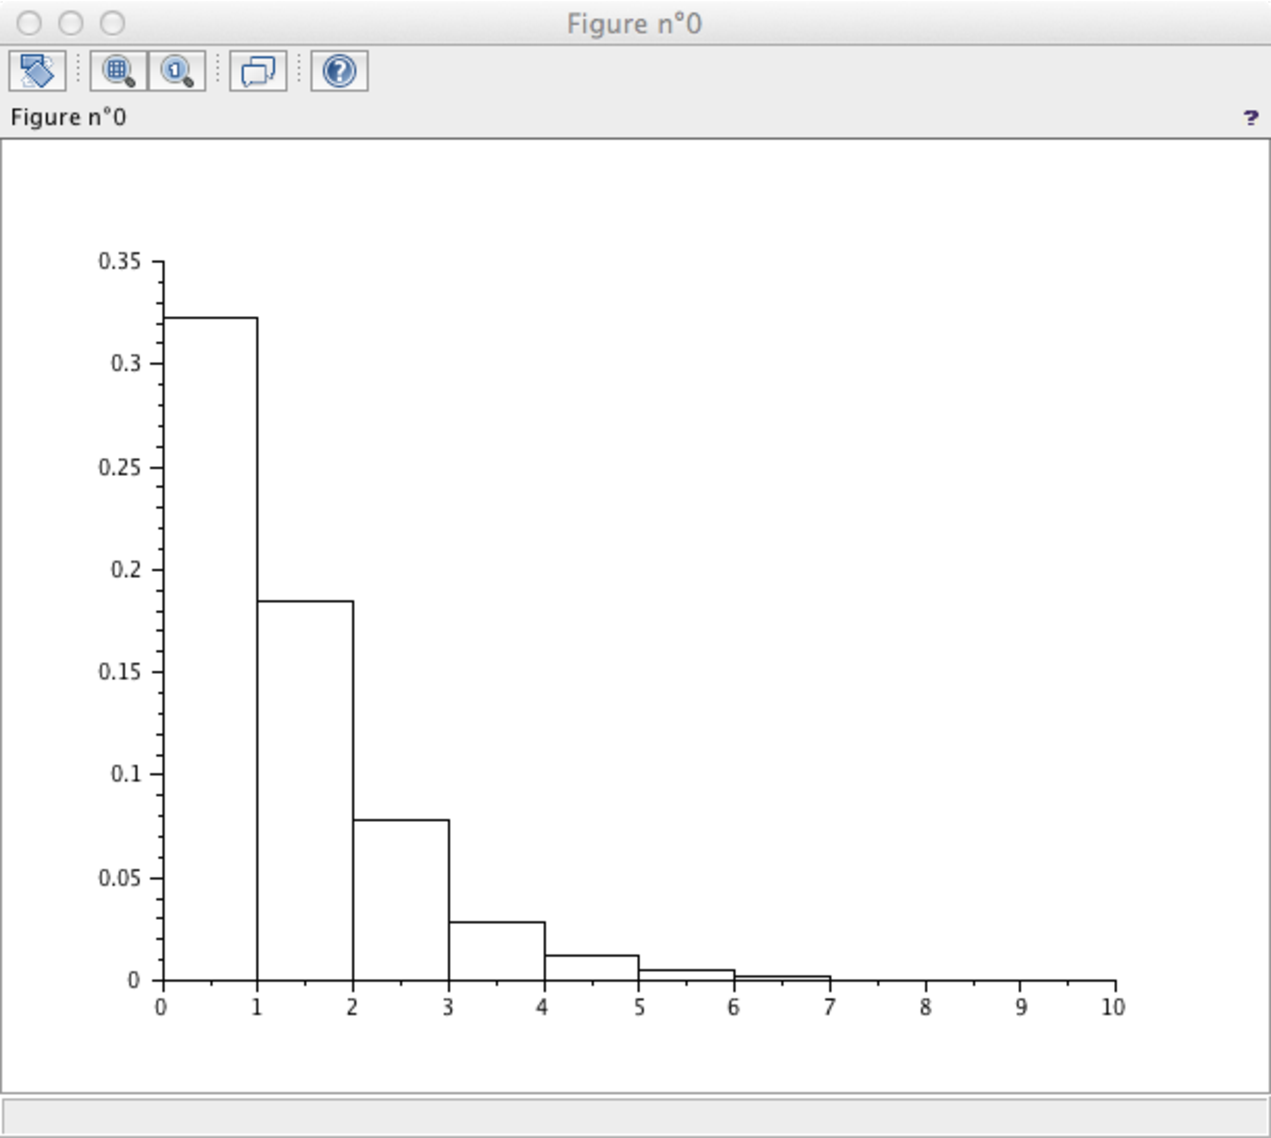
\includegraphics[width = 6cm,height =
    6cm]{Figures/EDHEC_2017/loi_faible_EDHEC_2017.pdf} & 
    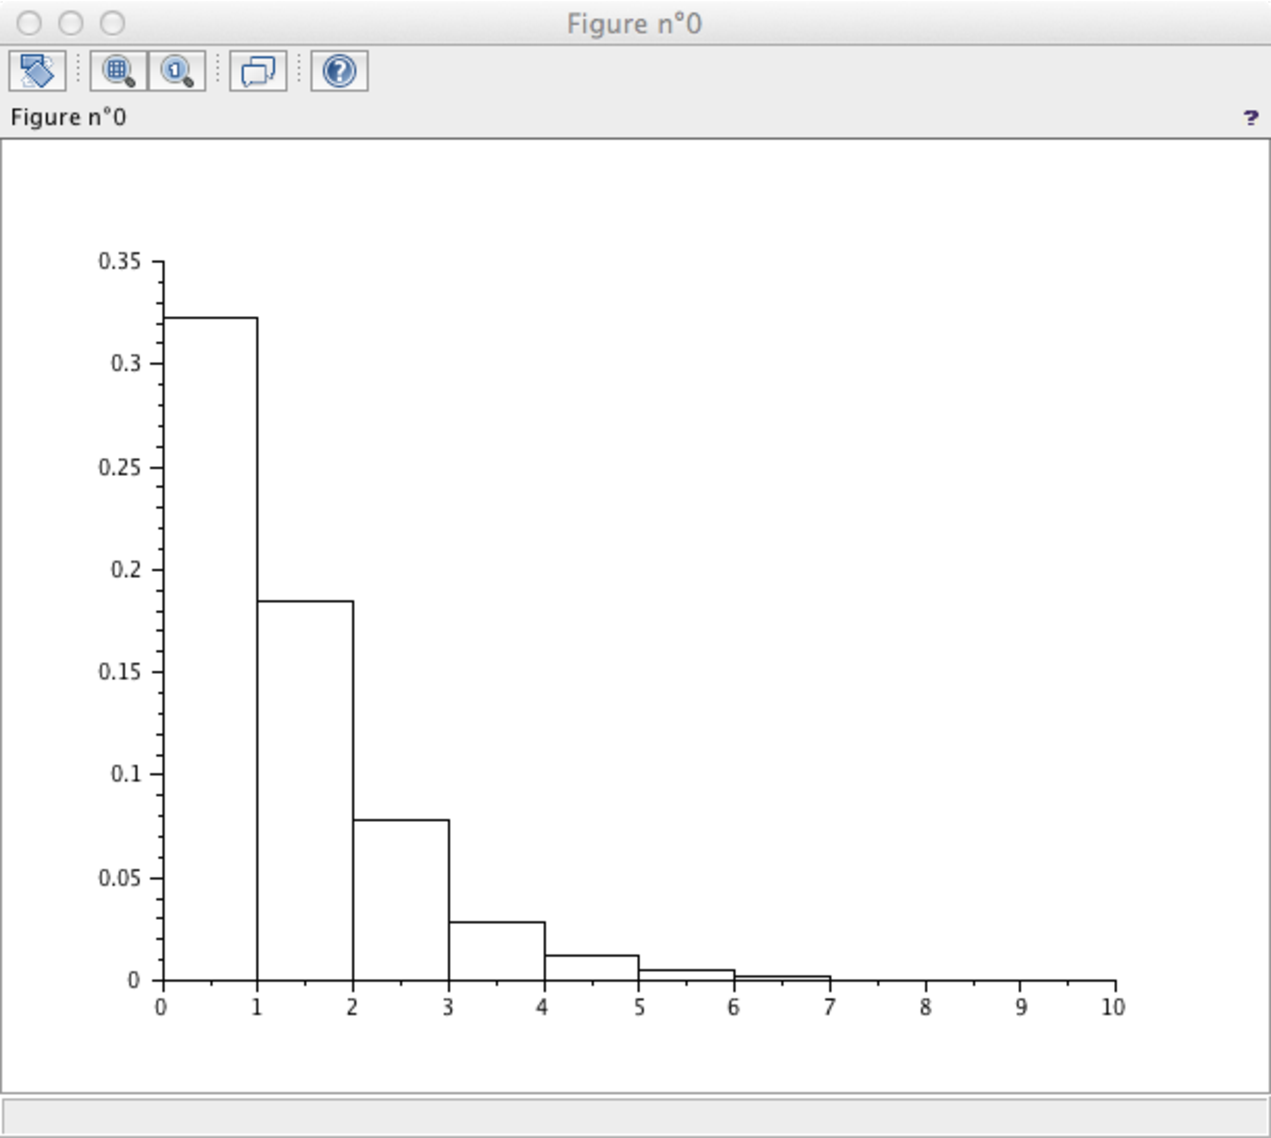
\includegraphics[width = 6cm,height =
    6cm]{Figures/EDHEC_2017/loi_faible_EDHEC_2017.pdf} \nl 
    Histogramme (1) & Histogramme (2) pour $n = 1000$
  \end{array}
  \]
  Quelle conjecture peut-on émettre quant au comportement de la suite
  des \var $(Z_{n})$ ?

  
\end{noliste}


%\newpage


\item On note $F_{Z_{n}}$ la fonction de répartition de $Z_{n}$.
  \begin{noliste}{a)}
    \setlength{\itemsep}{2mm}
  \item Justifier que, pour tout réel $x$, on a : $F_{Z_{n}}(x) =
    F_{Y_{n}}\left(x + \ln(n)\right)$.
    
    

  \item Déterminer explicitement $F_{Z_{n}}(x)$.
  
  
  

  %\newpage


  \item Montrer que, pour tout réel $x$, on a : $ \dlim{n \to +
      \infty} n \ln\left(1-\dfrac{\ee^{-x}}{n} \right) = -\ee^{-x}$.
      
      
      
  \item Démontrer le résultat conjecturé à la question \itbf{5.b)}.
  
    
  \end{noliste}
\end{noliste}


\newpage


\section*{Problème}

\subsection*{Partie 1 : étude d'une variable aléatoire}

\noindent
Les sommets d'un carré sont numérotés 1, 2, 3, et 4 de telle façon que
les côtés du carré relient le sommet 1 au sommet 2, le sommet 2 au
sommet 3, le sommet 3 au sommet 4 et le sommet 4 au sommet 1.\\
Un mobile se déplace aléatoirement sur les sommets de ce carré selon
le protocole suivant :
\begin{noliste}{$\sbullet$}
\item Au départ, c'est à dire à l'instant $0$, le mobile est sur le
  sommet 1.
\item Lorsque le mobile est à un instant donné sur un sommet, il se
  déplace à l'instant suivant sur l'un quelconque des trois autres
  sommets, et ceci de façon équiprobable.
\end{noliste}
Pour tout $n \in \N$, on note $X_{n}$ la variable aléatoire égale au
numéro du sommet sur lequel se situe le mobile à l'instant
$n$. D'après le premier des deux points précédents, on a donc $X_{0} =
1$.
\begin{noliste}{1.}
  \setlength{\itemsep}{4mm}
\item Donner la loi de $X_{1}$, ainsi que l'espérance $\E(X_{1})$ de
  la variable $X_{1}$.

  
  On admet pour la suite que la loi de $X_{2}$ est donnée par :
  \[
  \Prob\left(\Ev{X_{2} = 1}\right) = \dfrac{1}{3}, \quad
  \Prob\left(\Ev{X_{2} = 2}\right) = \Prob\left(\Ev{X_{2} = 3}\right)
  = \Prob\left(\Ev{X_{2} = 4}\right) = \dfrac{2}{9}
  \]


  %\newpage


\item Pour tout entier $n$ supérieur ou égal à 2, donner, en
  justifiant, l'ensemble des valeurs prises par $X_{n}$.

  

\item
  \begin{noliste}{a)}
    \setlength{\itemsep}{2mm}
  \item Utiliser la formule des probabilités totales pour établir que,
    pour tout entier naturel $n$ supérieur ou égal à 2, on a :
    \[
    \Prob\left(\Ev{X_{n + 1} = 1}\right) =
    \dfrac{1}{3}\left(\Prob\left(\Ev{X_{n} = 2}\right) + \Prob\left(\Ev{X_{n}
          = 3}\right) + \Prob\left(\Ev{X_{n} = 4}\right)\right)
    \]

    

  \item Vérifier que cette relation reste valable pour $n = 0$ et $n =
    1$.

    

  \item Justifier que, pour tout $n$ de $\N$, on a $\Prob(\Ev{X_{n} =
      1}) + \Prob(\Ev{X_{n} = 2}) + \Prob(\Ev{X_{n} = 3}) +
    \Prob(\Ev{X_{n} = 4}) = 1$ et en déduire l'égalité :
    \[
    \forall n \in \N, \ \Prob\left(\Ev{X_{n + 1} = 1}\right) =
    -\dfrac{1}{3} \ \Prob\left(\Ev{X_{n} = 1}\right) + \dfrac{1}{3}
    \]

    


    %\newpage


  \item Établir alors que : $\forall n \in \N, \ \Prob\left(\Ev{X_{n}
        = 1}\right) = \dfrac{1}{4} +
    \dfrac{3}{4}\left(-\dfrac{1}{3}\right)^{n}$.

    
  \end{noliste}
  

%\newpage


\item
  \begin{noliste}{a)}
    \setlength{\itemsep}{2mm}
  \item En procédant de la même façon qu'à la question précédente,
    montrer que l'on a :
    \[
    \forall n \in \N, \ \Prob\left(\Ev{X_{n + 1} = 2}\right) =
    \dfrac{1}{3} \ \left( \Prob\left(\Ev{X_{n} = 1}\right) +
      \Prob\left(\Ev{X_{n} = 3}\right) + \Prob\left(\Ev{X_{n} =
          4}\right)\right)
    \]

    

  \item En déduire une relation entre $\Prob\left(\Ev{X_{n + 1} =
        2}\right)$ et $\Prob\left(\Ev{X_{n} = 2}\right)$.

    


    %\newpage


  \item Montrer enfin que : $\forall n \in \N, \Prob\left(\Ev{X_{n} =
        2}\right) = \dfrac{1}{4} - \dfrac{1}{4} \
    \left(-\dfrac{1}{3}\right)^{n}$.

    

  \end{noliste}
  
\item On admet que, pour tout entier naturel $n$, on a :
  \[
  \Prob\left(\Ev{X_{n + 1} = 3}\right) = -\dfrac{1}{3} \ 
  \Prob\left(\Ev{X_{n} = 3}\right) + \dfrac{1}{3} \quad \hbox{ et }
  \quad \Prob\left(\Ev{X_{n + 1} = 4}\right) = -\dfrac{1}{3} \ 
  \Prob\left(\Ev{X_{n} = 4}\right) + \dfrac{1}{3}
  \]
  En déduire sans calcul que :
  \[
  \forall n \in \N, \ \Prob\left(\Ev{X_{n} = 3}\right) =
  \Prob\left(\Ev{X_{n} = 4}\right) =
  \dfrac{1}{4}-\dfrac{1}{4}\left(-\dfrac{1}{3}\right)^{n}
  \]

  


  %\newpage

  
\item Déterminer, pour tout entier naturel $n$, l'espérance
  $\E(X_{n})$ de la variable aléatoire $X_{n}$.

  

\end{noliste}


\newpage


\subsection*{Partie 2 : calcul des puissances d'une matrice $A$}

\noindent
Pour tout $n$ de $\N$, on considère la matrice-ligne de $\M{1,4}$ :
\[
U_{n} =
\begin{smatrix}
  \Prob\left(\Ev{X_{n} = 1}\right) & \Prob\left(\Ev{X_{n} = 2}\right)
  & \Prob\left(\Ev{X_{n} = 3}\right) & \Prob\left(\Ev{X_{n} =
      4}\right)
\end{smatrix}
\]
\begin{noliste}{1.}
  \setlength{\itemsep}{4mm}%
 \setcounter{enumi}{6}
\item 
  \begin{noliste}{a)}
    \setlength{\itemsep}{2mm}
  \item Montrer (grâce à certains résultats de la partie 1) que, si
    l'on pose $A = \dfrac{1}{3}\begin{smatrix}
      0 & 1 & 1 & 1\\
      1 & 0 & 1 & 1\\
      1 & 1 & 0 & 1\\
      1 & 1 & 1 & 0
    \end{smatrix}
    $, on a :  
    \[
    \forall n \in \N, \ U_{n + 1} = U_{n} \ A 
    \]

    

  \item Établir par récurrence que : $\forall n \in \N, \ U_{n} =
    U_{0} \ A^{n}$.

    

  \item En déduire la première ligne de $A^{n}$.

    
  \end{noliste}
  
  
  %\newpage
  
  
\item Expliquer comment choisir la position du mobile au départ pour
  trouver les trois autres lignes de la matrice $A^{n}$, puis écrire
  ces trois lignes.

  
\end{noliste}

% 


%\newpage


\subsection*{Partie 3 : une deuxième méthode de calcul des puissances
  de $A$}

\noindent
On considère les matrices $I$ et $J$ suivantes : $I =
\begin{smatrix}
  1 & 0 & 0 & 0\\
  0 & 1 & 0 & 0\\
  0 & 0 & 1 & 0\\
  0 & 0 & 0 & 1
\end{smatrix}
$ et $J = 
\begin{smatrix}
  1 & 1 & 1 & 1\\
  1 & 1 & 1 & 1\\
  1 & 1 & 1 & 1\\
  1 & 1 & 1 & 1
\end{smatrix}
$.
\begin{noliste}{1.}
  \setlength{\itemsep}{4mm}%
  \setcounter{enumi}{8}
\item Déterminer les réels $a$ et $b$ tels que $A = aI + bJ$.

  

\item
  \begin{noliste}{a)}
    \setlength{\itemsep}{2mm}
  \item Calculer $J^{2}$ puis établir que, pour tout entier naturel
    $k$ non nul, on a : $J^{k} = 4^{k-1} J$.

    

  \item À l'aide de la formule du binôme de Newton, en déduire, pour
    tout entier $n$ non nul, l'expression de $A^{n}$ comme combinaison
    linéaire de $I$ et $J$.

    

  \item Vérifier que l'expression trouvée reste valable pour $n = 0$.

    
  \end{noliste}
\end{noliste}

\subsection*{Partie 4 : informatique}

\begin{noliste}{1.}
  \setlength{\itemsep}{4mm}%
  \setcounter{enumi}{10}
\item
  \begin{noliste}{a)}
    \setlength{\itemsep}{2mm}
  \item Compléter le script \Scilab{} suivant pour qu'il affiche les
    100 premières positions autres que celle d'origine, du mobile dont
    le voyage est étudié dans ce problème, ainsi que le nombre $n$ de
    fois où il est revenu sur le sommet numéroté 1 au cours de ses 100
    premiers déplacements (on pourra utiliser la commande {\tt sum}).
    \begin{scilab}
      & A = [------] / 3 \nl %
      & x = grand(100,\ttq{}markov\ttq{},A,1) \nl %
      & n = ------ \nl %
      & disp(x) \nl %
      & disp(n) \nl %
    \end{scilab}


    %\newpage


    


    %\newpage


  \item Après avoir exécuté cinq fois ce script, les réponses
    concernant le nombre de fois où le mobile est revenu sur le sommet
    1 sont : $n = 23$, $n = 28$, $n = 23$, $n = 25$, $n = 26$.\\
    En quoi est-ce normal ?

    
  \end{noliste}
\end{noliste}


%\newpage




